%%%%%%%%%%%%%%%%%%%%%%%%%%%%%%%%%%%%%%%%%
% University Assignment Title Page 
% LaTeX Template
% Version 1.0 (27/12/12)
%
% This template has been downloaded from:
% http://www.LaTeXTemplates.com
%
% Original author:
% WikiBooks (http://en.wikibooks.org/wiki/LaTeX/Title_Creation)
%
% License:
% CC BY-NC-SA 3.0 (http://creativecommons.org/licenses/by-nc-sa/3.0/)
% 
% Instructions for using this template:
% This title page is capable of being compiled as is. This is not useful for 
% including it in another document. To do this, you have two options: 
%
% 1) Copy/paste everything between \begin{document} and \end{document} 
% starting at \begin{titlepage} and paste this into another LaTeX file where you 
% want your title page.
% OR
% 2) Remove everything outside the \begin{titlepage} and \end{titlepage} and 
% move this file to the same directory as the LaTeX file you wish to add it to. 
% Then add \input{./title_page_1.tex} to your LaTeX file where you want your
% title page.
%
%%%%%%%%%%%%%%%%%%%%%%%%%%%%%%%%%%%%%%%%%
%\title{Title page with logo}
%----------------------------------------------------------------------------------------
%	PACKAGES AND OTHER DOCUMENT CONFIGURATIONS
%----------------------------------------------------------------------------------------

\documentclass[12pt]{article}
\usepackage[english]{babel}
\usepackage[utf8x]{inputenc}
\usepackage{amsmath}
\usepackage{graphicx}
\usepackage[top=2.5cm, bottom=3cm, left=2.5cm, right=2.5cm]{geometry}
\usepackage[colorinlistoftodos]{todonotes}
\setcounter{tocdepth}{3} 
\setcounter{secnumdepth}{3}


\begin{document}

\begin{titlepage}

\newcommand{\HRule}{\rule{\linewidth}{0.5mm}} % Defines a new command for the horizontal lines, change thickness here

\center % Center everything on the page
 
%----------------------------------------------------------------------------------------
%	HEADING SECTIONS
%----------------------------------------------------------------------------------------
\centering
\includegraphics[height=3cm]{logofac.png}\\[1.5cm]


%----------------------------------------------------------------------------------------
%	TITLE SECTION
%----------------------------------------------------------------------------------------

\HRule \\[0.6cm]
{ \huge \bfseries Projet Moriarty}\\[0.4cm] % Title of your document
\HRule \\[0.6cm]

\vfill
\centering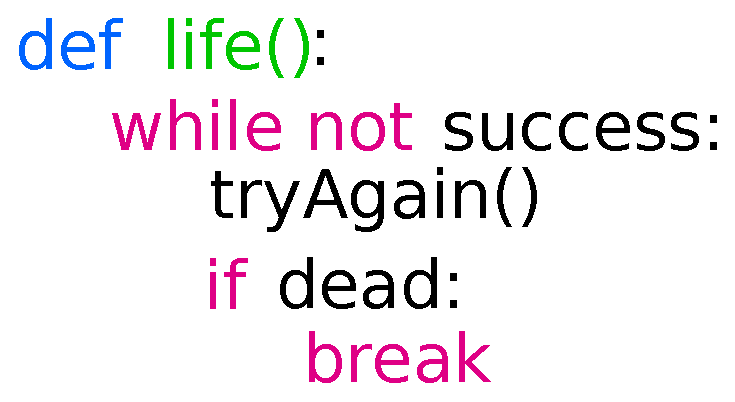
\includegraphics[height=6cm]{joke.eps}\\[0.5cm]
\vfill

%----------------------------------------------------------------------------------------
%	AUTHOR SECTION
%----------------------------------------------------------------------------------------


% If you don't want a supervisor, uncomment the two lines below and remove the section above
\Large \emph{Auteurs:}\\
Thomas \textsc{MAUCOURT}\\[0.1cm] % Your name
Adrien \textsc{MENDES SANTOS}\\[1cm] % Your name

%----------------------------------------------------------------------------------------
%	DATE SECTION
%----------------------------------------------------------------------------------------

{\large 23 Novembre 2016}\\[2cm] % Date, change the \today to a set date if you want to be precise


\end{titlepage}

%----------------------------------------------------------------------------------------
%	TABLE OF CONTENTS
%----------------------------------------------------------------------------------------

\setcounter{page}{0}
\thispagestyle{empty}
\tableofcontents
\newpage
 
\section{Introduction}

Le rapport suivant traite de la réalisation d'un projet consistant au développement d'un jeu appelé \verb|Moriarty ou la swing-protéine|. Ce projet s'inscrit dans le cadre de notre formation en Master 1 Bio-informatique mention Biologie Computationnelle. Il s'agit du premier projet de groupe que nous avions à réaliser. Ce projet avait pour objectif de nous sensibiliser au travail de programmation en équipe, en plus de nous fournir un entraînement conséquent dans la programmation en langage Python. Le projet imposé devait être réalisé dans un délai de 15 jours, un rapport au format PDF issu d'un document LaTeX devait être rendu au terme du délai. Dans les pages suivantes, nous proposons la description des différentes étapes que nous avons suivi afin d'aboutir à un programme fonctionnel.\\


\emph{Moriarty ou la swing-protéine} est un jeu de réflexion, se composant d'un plateau de jeu et de 64 pions bicolores (une face rouge, l'autre verte), portant sur l'activation ou l'inhibition d'une protéine ou d'un complexe protéique. Ce jeu offre la possibilité de jouer à deux joueurs ou bien à un joueur qui affrontera alors l'ordinateur. À partir de deux protéines pour chaque joueur (deux protéines activées et deux protéines inactivées) placées au centre du plateau de jeu, les joueurs doivent placer leurs pions de façon à changer l'état des protéines adverses, en respectant différentes règles ; la finalité étant d'avoir le plus de protéines activées ou inactivées selon le camp à la fin d'une partie.
\\Ce rapport sera divisé en trois grandes parties :
\begin{enumerate}
	\item Règles du jeu : nous expliquerons ici les règles du jeu qui ont été implémentées au sein du programme
	\item Conception : dans cette partie nous détaillerons les différentes étapes préalables de conception
	\item Réalisation : cette partie expliquera les différentes fonctions et algorithmes utilisés afin de produire un jeu fonctionnel
\end{enumerate}

Le jeu du Moriarty est disponible dans le dossier :\\ \\
\verb|/net/stockage/bioinfo2016/MAUCOURT_MENDES\Moriarty|\\
Le dossier Moriarty contient le fichier principal \verb|Moriart.py| ainsi qu'un dossier \verb|src|. Celui-ci comporte les fichiers \verb|Functions.py| et \verb|Data.py| regroupant les différentes fonctions et données nécessaires au fonctionnement du programme. Chaque fonctions ont été documentées en anglais.
\newpage
\section{Les règles du Jeu}

\subsection{But du jeu}

Les pions verts représentent les protéines actives, les pions rouges quant à eux représentent les protéines inactives. Les joueurs disposent d'un pot commun de 64 pions (correspondant à la taille du plateau de jeu). Si un pion est joué par l’activateur, ce pion prend la couleur verte, si c’est l’inhibiteur il prendra la couleur rouge. Les pions protéines peuvent changer d’état suivant leur environnement selon les règles décrites plus bas. Il est à noter que lors du tour d'un joueur, ce dernier est dans l'obligation de jouer un pion. La partie se termine  ainsi lorsque plus aucun mouvement n'est possible. Le vainqueur du jeu est celui possédant le plus grand nombre de pions de sa couleur à la fin de la partie.


\subsection{Les différents mouvements possibles}

Au début de la partie, quatre pions sont placés au centre du plateau afin d'y former un carré avec des pions de couleurs alternées (par exemple un vert et un rouge, puis un rouge et un vert dans la ligne du dessous).
% Mettre schéma ?
À son tour de jeu, le joueur doit poser un pion de sa couleur à une position autorisée.
\\Il est nécessaire de respecter deux conditions afin qu'une position soit autorisée:
\begin{enumerate}
\item Un joueur ne peut pas poser son pion sur une case déjà occupée par un autre pion, et cela peu importe sa couleur.
\item Le placement du pion doit induire un changement d'état d'au minimum un pion adverse.

\end{enumerate}

La première condition étant assez explicite nous ne la détaillerons pas. La deuxième, quant à elle, mérite quelques précisions. Lorsque deux pions d'une même couleur encadrent un ou plusieurs pions en respectant la première condition, il se produit un changement d'état des protéines de tel sorte que tous les pions qui sont contenus dans cet encadrement changent d'état.
\\\emph{La Figure 1} donne un exemple des différents mouvements autorisés ou non.
\\


\begin{figure}
	\begin{center}
	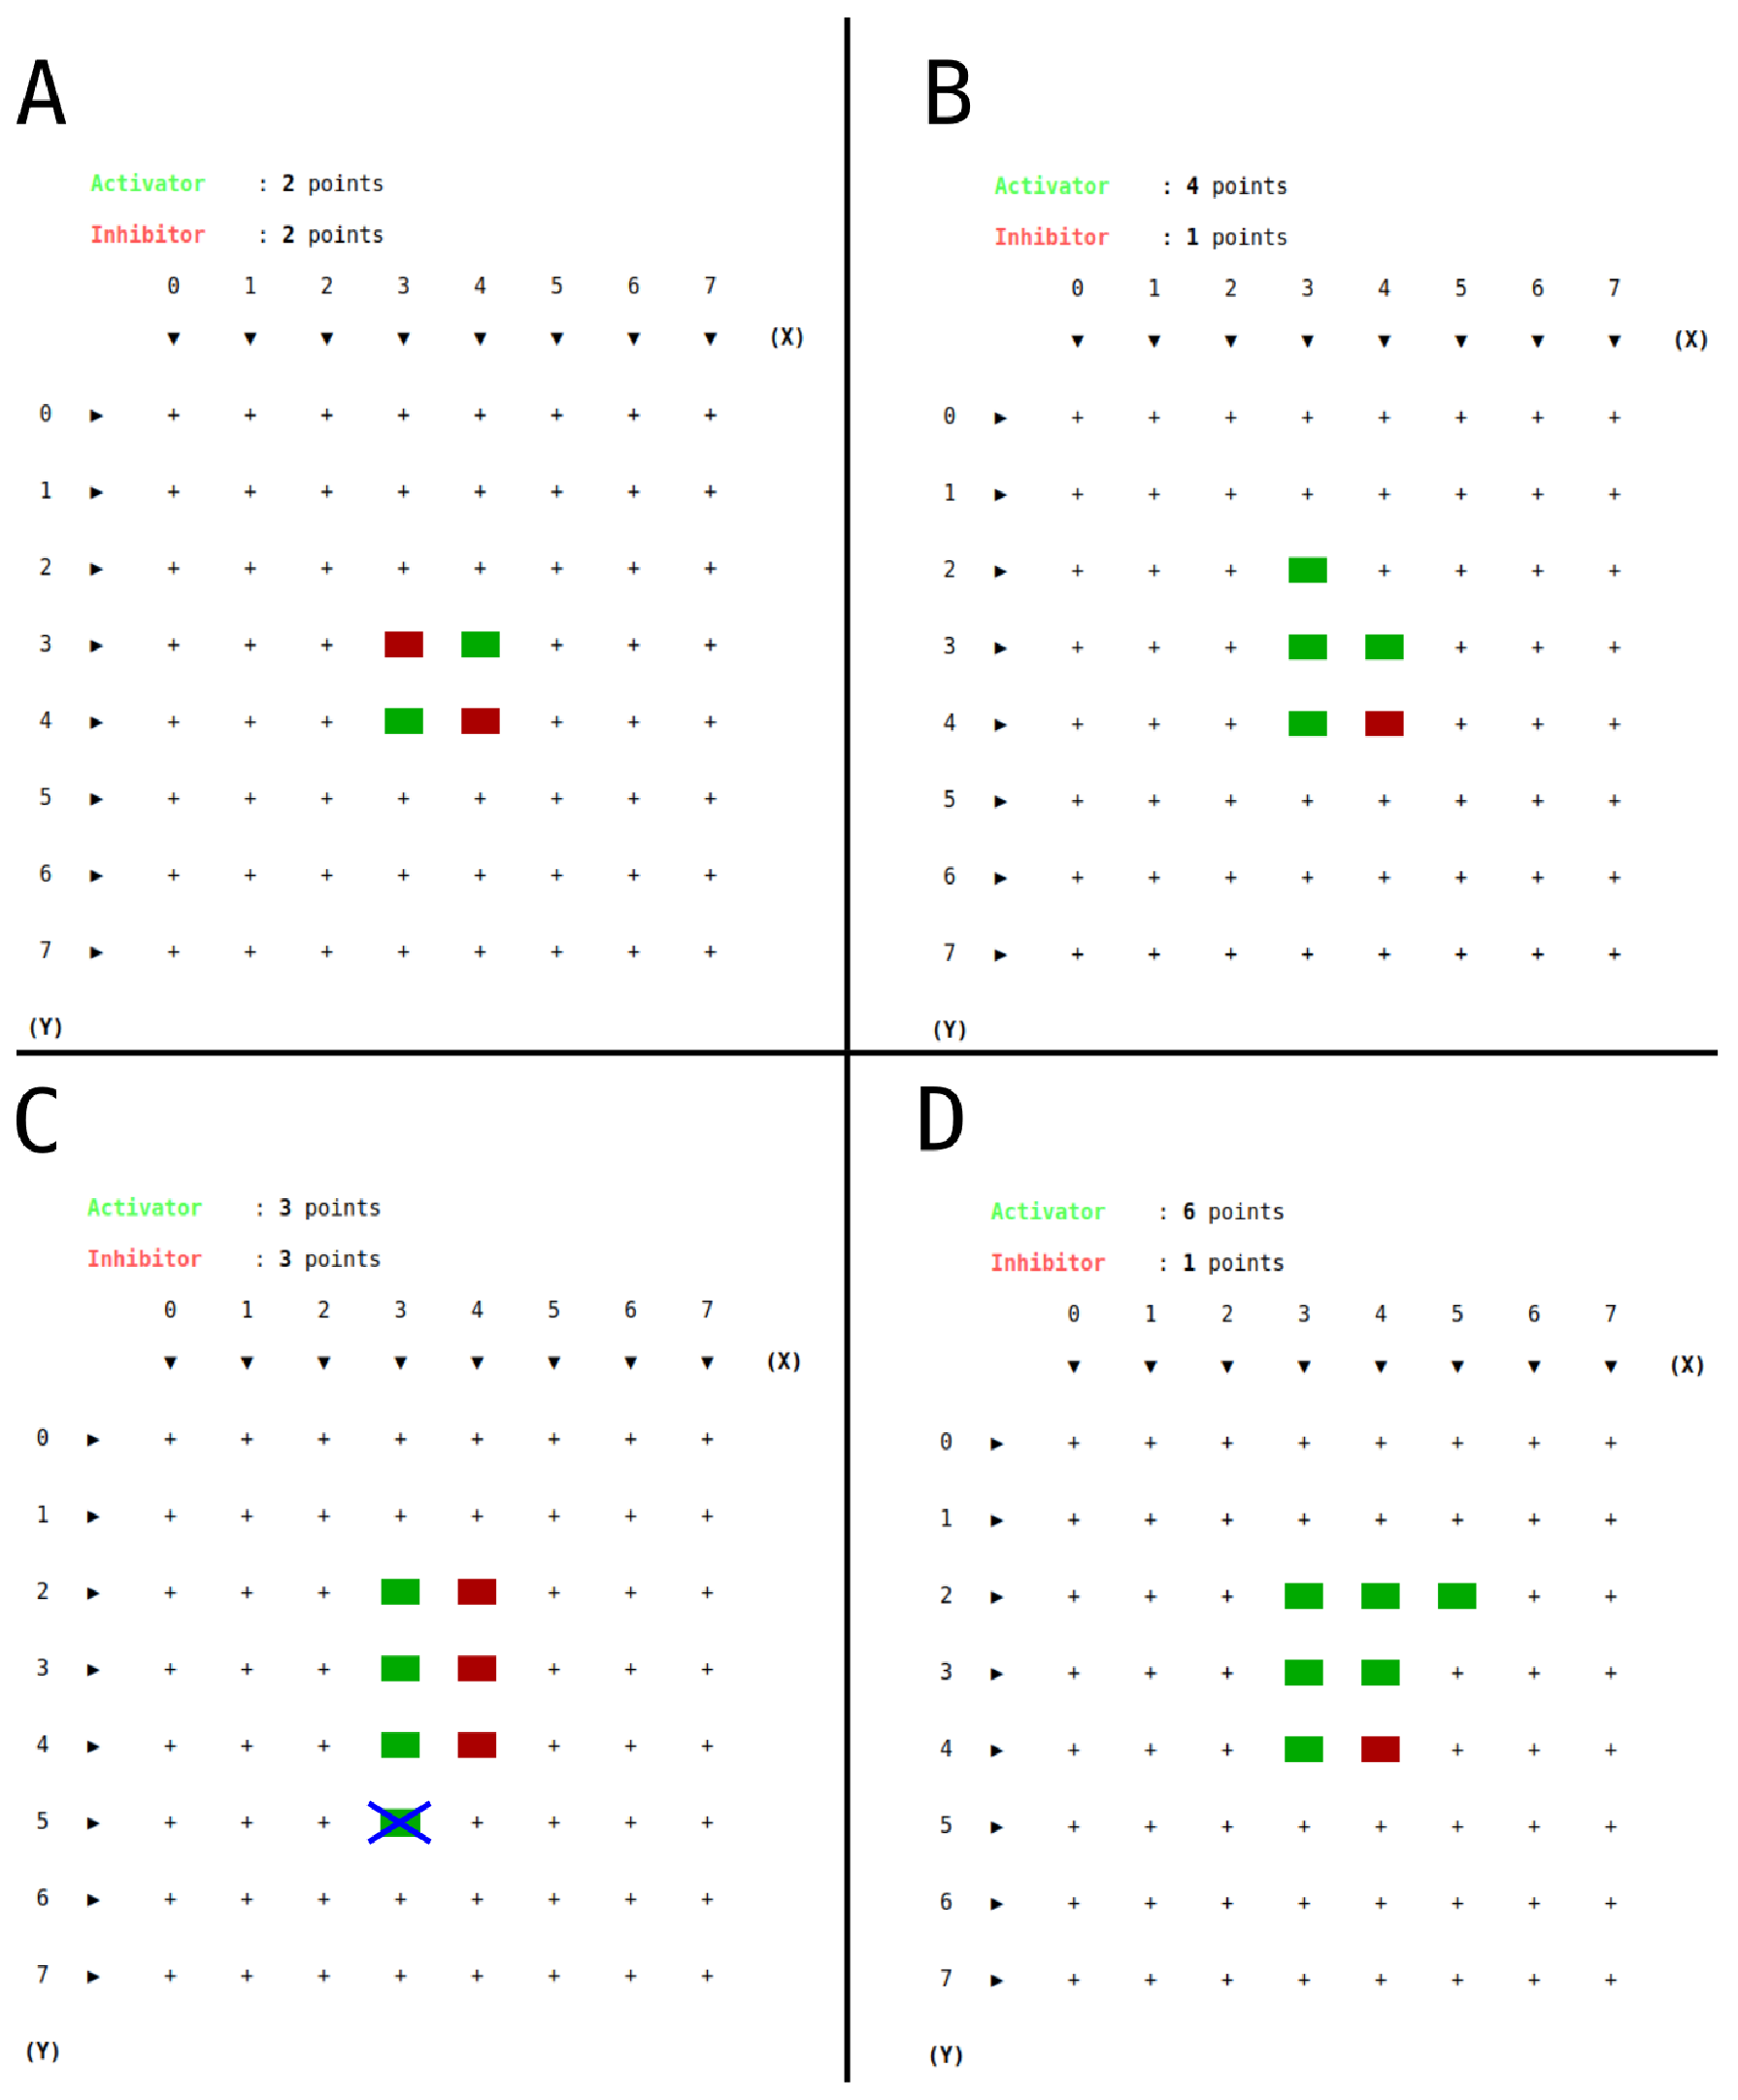
\includegraphics[scale=0.52]{fig1.eps}
	\end{center}
	\caption{\small{\textbf{Illustration des mouvements autorisés.} \textbf{A.} Initialisation du plateau de jeu. \textbf{B.} Dépôt d'un pion vert en (3,2) entraînant un changement d'état du pion rouge en (3,3). \textbf{C.} Tentative de dépôt d'un pion vert en (3,5) qui n'aboutit pas, du fait de coordonnées ne respectant pas la règle numéro 2. \textbf{D. } Dépôt d'un pion vert en (5,2) induisant un changement des pions rouges situés en (4,2) \& (4,3)}}
\end{figure}


\section{La Conception du Jeu}

Avant de commencer le travail de développement en Python sur ordinateur du jeu Moriarty, nous avons commencé par une étape initiale de réflexion. Au cours de cette phase, nous avons posé sur papier, non pas un début de code, mais plutôt les différentes étapes du déroulement du jeu sous forme de pseudocode. Ceci dans le but de n'avoir au final plus qu'à implémenter nos différents algorithmes.
\\Lorsque nous rencontrions des difficultés pendant la phase de développement, nous avons réitéré ce travail de réflexion afin de comprendre les subtilités qui nous auraient échappé.
\\Cette phase de conception a ainsi eu une importance, selon nous, non négligeable. Nous partagerons les éléments de cette dernière dans cette partie.

\subsection{Le plateau de jeu}

Comme expliqué dans les règles, le jeu de \verb|Moriarty ou la swing-protéine| se joue sur un plateau de 64 cases.
\\Nous avons dû ainsi créer un plateau de jeu. Pour cela nous avons adopté une stratégie consistant à utiliser des coordonnées pour chaque case, ainsi que le contenu de cette case à un instant donné. Ce plateau est ensuite mis à jour après chaque mouvement.

\subsection{Calcul des différents mouvements possibles}

Cette partie a été l'élément central et le plus complexe à développer. En effet, pour rappel, un pion ne peut être joué que si ce dernier ne prend pas la place d'un autre pion. Par ailleurs, ce mouvement doit également induire un changement d'état pour qu'il soit validé.
\\Il nous a ainsi fallu développer un algorithme permettant de vérifier toutes les cases adjacentes au pion posé. Cet algorithme devait aussi permettre de déterminer si le placement de ce pion à ces coordonnées, pouvait induire un changement d'état d'au moins une protéine.
\\Au cours de l'étape de développement de l'algorithme, nous nous sommes heurtés à différents problèmes techniques. En effet, dans un premier temps nous avons décidé de partir d'un cas simple, à savoir la possibilité de modifier un pion adverse uniquement si celui-ci était encadré par 2 pions de la même couleur. Cette étape de développement a été relativement simple. Le problème est apparu quand nous avons dû prendre en compte la possibilité de changer l'état de plusieurs pions dans une même direction. En effet l'utilisation de l'algorithme développé précédemment nous l'aurait permis mais cela au détriment d'un code lisible et simple. Ainsi nous avons dû adopter une autre stratégie détaillée plus tard dans ce rapport.

\subsection{L'intelligence artificielle}


Malgré le fait que la réalisation d'une Intelligence Artificielle (IA) était une partie optionnelle, nous avons décidé de nous lancer dans ce défi technique. En effet cela nous a paru plus intéressant d'avoir la possibilité de jouer contre une IA en cas d'absence de partenaire réel.
\\Avant de commencer l'étape de conception, nous n'avions qu'une très vague idée de la façon dont nous ferions fonctionner cette IA. Celle-ci étant un objectif secondaire, nous avons préféré nous lancer dans le développement du cœur du jeu avant de nous pencher sur cette option.
\\Néanmoins, une fois la partie centrale du jeu développée, nous avons pu nous intéresser plus particulièrement à cet objectif. Ainsi nous avons pu développer cette IA assez rapidement au vu de la structuration de notre code. Tous les problèmes que nous pensions rencontrer durant le développement de l'IA ont disparu une fois les fonctions principales développées. En effet, ces fonctions utilisées lors d'une partie traditionnelle (opposant un humain à un autre) pouvaient tout à fait être "adaptées" afin d'insérer la possibilité à une IA de prendre la place d'un joueur humain lors d'une partie.
\newpage
Au vu du fonctionnement de nos fonctions, nous avons pu nous permettre de développer 2 niveaux distincts d'IA :
\begin{itemize}
	\item \emph{IA de niveau Normal} : IA se contentant de tirer une position aléatoire au sein de positions autorisées pour le placement d'un pion.
	\item \emph{IA de niveau Difficile} : IA calculant le coup permettant l'obtention du plus de pions lors du mouvement. L'appellation "Difficile" de cette IA n'est pas représentative de la réalité. En effet, dans certains cas, l'utilisation de ce type d'algorithme de maximisation du nombre de pions à prendre n'est pas forcément le meilleur du fait que cette IA ne se limite qu'aux données qu'elle possède à un moment donné, et ne prend pas en compte les tours suivants.
\end{itemize}

Cette étape de la conception nous a permis de réfléchir plus profondément aux concepts de ce jeu, et nous a permis de mieux comprendre la complexité que pouvait avoir la programmation d'une IA ayant la possibilité de prévoir plusieurs manches en avance. La méthode de développement de ces différentes IA est détaillée plus tardivement dans ce rapport.

\subsection{Les détails qui font une différence}

Avant de passer à l'étape de la conception, nous avons réalisé que nous devions aussi réfléchir à différents détails, afin de rendre notre jeu le plus personnel possible.
\\C'est ainsi, que nous nous sommes accordé sur le fait qu'il nous fallait déjà envisager une des propositions optionnelles. N'ayant, chacun de nous, que peu d'expérience dans l'implémentation d'interfaces graphiques, et le délai imposé ne nous permettant pas d'acquérir suffisamment d'expérience, nous avons éliminé cette option.
\\Toutefois, afin de compenser la "perte" de cette option, nous avons décidé d'implémenter différentes options qui trouvent une utilité que nous avons jugé importante :

\begin{itemize}
	\item \emph{Menu principal} : un menu permettant la navigation au sein de notre programme et jouant le rôle d'interface graphique rudimentaire.
	\item \emph{Mode Daltonien} : un mode qui nous a semblé important d'implémenter au vu de la forte proportion de personne atteinte de daltonisme au sein de la population mondiale (~8\% de le population masculine mondiale, les femmes étant moins touchées).
\end{itemize}
%Par ailleurs, par souci de confort, les scores des différents joueurs sont sauvegardés dans un fichier CSV et lors d'une nouvelle partie, le joueur peut accéder à son historique de scores.

\newpage
\section{La Réalisation du Jeu}

Au cours de cette partie nous nous concentrerons sur la partie développement du projet. Nous expliquerons de quelles façons nous avons traduit les différents objectifs que nous avions déterminés durant la phase de conception, en langage de programmation Python 3.5 afin d'obtenir un jeu fonctionnel.

\subsection{Le menu }

Le lancement du script \verb|Moriarty.py| mène l’utilisateur au menu principal à l'aide de la fonction  \textit{display\_menu()}. Plusieurs choix s'offrent à lui :
\begin{itemize}
\item Afficher les règles du jeu
\item Joueur vs Joueur
\item Joueur vs Ordinateur  
\item Mode d'affichage (Mode normal ou mode daltonien)
\item Quitter
\end{itemize}


\subsection{Le plateau de jeu }

Comme vu précédemment, nous devions créer un plateau de jeu dans lequel chaque case est définis par des coordonnées de type (x,y).
L'affichage graphique du plateau est réalisé à l'aide de la fonction \textit{display\_grid()}. La première ligne et colonne sont composées des différents axes X et Y. La deuxième ligne / colonne, d'un caractère ASCII représentant une flèche afin que l'utilisateur puisse facilement associer les positions X et Y aux lignes et colonnes correpondantes (\textit{cf} Figure 1). L'affichage de la grille a été réalisée par l'utilisation de boucles for du fait de la structure de notre plateau, mais également pour simplifier le code.
Les coordonnées étant des éléments fixes, nous avons opté pour les insérer dans des tuples. Ceux-ci sont compris dans un dictionnaire afin de pouvoir associer une coordonnée, qui prend ici le rôle de clé, et le statut de cette case (ce qu'elle contient) qui prend ici le rôle de valeur du dictionnaire.
\\L'initialisation du plateau composée des deux premiers pions activateurs et des deux premiers pions inhibiteurs est réalisée à l'aide de la fonction \textit{create\_initial\_grid()} qui va se charger de créer le dictionnaire avec les 4 pions de départ ainsi que les autres cases qui auront la valeur par défaut ' + '.
\\À chaque fois qu'un joueur sélectionne une position autorisée, la fonction \textit{update\_grid()} se charge de mettre à jour le plateau avec la nouvelle position et les différents changements induits par ce mouvement. Cette mise à jour est possible par la récupération de la fonction des différentes cases prises par le joueur courant. Une fois ces cases récupérées, une boucle permettant de parcourir le plateau permet de redéfinir les valeurs associées au coordonnées prises par la couleur du pion du joueur.
\\La fin de la partie est déterminée à l'aide de la fonction \textit{check\_end()} qui a pour rôle de vérifier s'il existe encore des mouvements possibles. Cette fonction se contente de simuler la pose d'un pion de la couleur du joueur courant dans toutes les cases du tableau. Dans le cas ou une des coordonnée utilisée peut entrainer la modification de statut d'au moins un pion, la partie continue. Dans le cas contraire la partie se termine et les scores sont calculées à l'aide de la fonction \textit{get\_score()}. Cette fonction va utiliser le même algorithme de parcours du plateau que la fonction précédente mais va cette fois-ci utiliser un compteur pour chaque joueur. Dans le cas ou la case est remplie par le couleur d'un des joueurs, le compteur correspondant est incrémenté. A la fin, les scores sont renvoyés. Le joueur ayant le plus haut score, correspondant à celui qui a le plus de pions de sa couleur sur le plateau, est désigné vainqueur.

\subsection{Joueurs et scores}

Aussi bien dans le mode joueur vs IA que joueur vs joueur, il est possible de choisir si le joueur souhaite jouer les activateurs ou les inhibiteurs (dans le cas du mode joueur vs IA), ou bien de décider le rôle de chaque joueur (pour le mode joueur vs joueur).
Ce processus est géré par la fonction \textit{create\_player()}, qui va de plus colorer le pseudo des joueurs ce qui permettra de rappeler à chaque joueur leur rôle au cours de la partie. Cette fonction permet de modifier les clés d'un dictionnaire généré par défaut en début de partie. Ce dictionnaire associe le nom d'un joueur avec la valeur de ses pions. La saisie du nom d'un joueur mène à la modification de la clé par défaut du dictionnaire correspondant au rôle du joueur (activateur ou inhibiteur).
\\Dans le jeu de \verb|Moriarty ou la swing-protéine|, les scores en cours de partie n'ont que peu de valeur étant donné qu'il est possible en un tour (d'activer ou d'inactiver) de gagner toute une ligne de protéines pour au prochain tour les reperdre. Néanmoins par soucis de visibilité, nous avons inclus un système de score en cours de partie. Celui-ci compte le nombre de protéines activées ainsi que les protéines inactivées pour ensuite afficher ces scores, tout ceci à l'aide de la fonction \textit{get\_score()}, l'algorithme a été décrit dans la partie précédente.

\subsection{Détermination des mouvements autorisés \& acquisition des pions}

L'écriture du code de cette partie a été l'élément central du programme.
\\En effet, c'est à ce moment que nous avons dû implémenter l'algorithme permettant de déterminer la validité du coup proposé par le joueur et permettant de récupérer les pions capturés lors du mouvement.
\\Nous avons ainsi implémenté plusieurs fonctions :
\begin{itemize}
	\item \emph{get\_position()} : Permet de tester les coordonnées entrées par le joueur. Pour cela, la fonction va vérifier si le joueur a bien entré des coordonnées valides dans le cadre de notre plateau (8x8). Cela consiste également à regarder si la case choisie est bien vide (' + '). Par la suite, cette fonction appelle une fonction \textit{check\_changes()} qui permet de calculer les différents changements induits.
	\item \emph{check\_changes()} : Permet de déterminer si les coordonnées entrées induisent au minimum un changement de statut d'une des cases du tableau. Cela est rendu possible par l'appel de la fonction \textit{get\_allowed\_position()}. Cette fonction va dans un premier temps récupérer l'ensemble des valeurs et coordonnées des points des lignes et diagonales autour de la case choisie par le joueur qu'elle va stocker dans 8 listes distinctes. Afin de faciliter le fonctionnement de \textit{check\_changes()}, ces listes sont réordonnées de telle sorte que les coordonnées aille de la case choisie vers l'extérieur du plateau de jeu. C'est sur ces listes ordonnées dans un sens précis que la fonction \textit{check\_changes()} va pouvoir travailler et ainsi récupérer les cases changeant de statut suite au mouvement choisis.
\end{itemize}

\subsection{La création de l'IA}

L'IA fonctionne à l'aide de trois fonctions que nous allons détailler ici :
\begin{itemize}
	\item \emph{IA\_creating\_players()} : Permet de créer les joueurs pour la partie. Le joueur aura le choix entre jouer le rôle d'activateur ou d'inhibiteur, l'IA aura le rôle opposé. Les différents rôles attribués modifient, comme dans le cas d'une partie joueur contre joueur, le dictionnaire contenant les rôles et valeurs de pions de la partie en cours. Au sein de cette fonction, le joueur pourra non seulement entrer son pseudo, choisir son rôle mais aussi définir le niveau de difficulté de l'IA (Normal ou Difficile).
	\item Les fonctions suivantes définissent la difficulté de l'IA qui est choisie lors de l'étape précédente :
	\begin{itemize}
		\item \emph{easy\_mode()} : Mode Normal de l'IA : Cette IA se contente de récupérer l'ensemble des positions jouables et en choisit une aléatoirement. L'algorithme est basé sur celui de la fonction \textit{check\_end()} à savoir que l'IA va dans un premier temps récupérer toutes les cases libres et simuler la pose de son pion sur ces cases. L'appel de la fonction \textit{check\_changes()} permet cette opération mais aussi de récupérer l'ensemble des cases menant à la prise d'au minimum 1 pion à l'adversaire. Un tirage aléatoire dans cette liste de coordonnées induisant un changement permet de définir la position que l'IA choisit. L'appel des fonctions utilisées par une partie joueur contre joueur permet ensuite de modifier la valeur des cases prises par l'IA.
		\item \emph{hardcore\_mode()} : Mode Difficile de l'IA : Cette fois-ci, l'algorithme de choix de position a été modifié. Comme précédemment le début consiste à simuler le positionnement sur toutes les cases libres du plateau. Par la suite est initié le calcul de la position rapportant le plus de pions. Cela consiste à récupérer la taille des différentes listes de positions prises en cas de choix de la position simulée. Cette IA est appelée "Difficile" mais comme décrit précédemment, ce mot est peu adapté à notre cas. 
	\end{itemize}		
	
\end{itemize}

\newpage

\section{Conclusions}
Le projet de création du jeu du \verb|Moriarty ou  la swing-protéine| a abouti à un logiciel fonctionnel. Néanmoins, le développement du jeu nous a amené à nous interroger plusieurs fois sur les stratégies à adopter afin de surmonter certains problèmes. Ainsi nous avons pu découvrir pour la première fois l'importance de la phase de réflexion sans utiliser d'ordinateur. Une fois notre projet analysé sur papier, il nous a été relativement simple d'implémenter nos différentes fonctions permettant l'aboutissement du projet. Ceci nous a conforté dans l'idée qu'utiliser cette approche est nécessaire au développement de programmes relativement importants en terme de lignes de code.


De plus ce projet nous a amené à découvrir le travail en groupe dans le cadre d'un travail de programmation. Cela nous a beaucoup apporté et nous avons beaucoup appris sur la manière de travailler en équipe sur un même projet informatique. Il nous a notamment amené à utiliser le site web \verb|https://www.github.com| ainsi qu'un des outils associé qu'est \verb|git|. Nous avons pu nous répartir les tâches et travailler chacun de notre coté durant la phase de développement (hors des réunions que nous avons eu afin de tester et de parler du projet). Ceci nous a permis de développer notre programme rapidement. \verb|Github| est un outils très puissant que nous avons beaucoup utilisé au cours de ce projet, il nous a permis de maintenir une version à jour de notre programme tout au long du développement. 


Le succès du projet, ne signifie pas qu'il n'y a pas de points à améliorer. Nous pourrions ainsi donner quelques idées de piste d'amélioration comme la réalisation d'une interface graphique à l'aide de bibliothèques telles que \verb|Tkinter| ou \verb|WxPython|, ce qui rendrait le jeu davantage "user friendly". Nous pourrions également implémenter la possibilité de sauvegarder une partie en cours afin de pouvoir la reprendre plus tardivement. Pour aller encore plus loin l'implémentation d'une couche réseau, permettant à des joueurs situés sur des machines différentes de jouer l'un contre l'autre, apporterait un gain important à notre programme. Cela permettrait de s'affranchir de la nécessité de jouer avec des personnes de notre entourage uniquement.\\


Notre travail est visible en ligne à l'adresse : \verb|https://github.com/Zarete/Moriarty|.\\

Vous trouverez un annexe un flowchart du programme \verb|Moriarty ou la swing-protéine| représentant les principales fonctions, et leurs interactions les unes entre les autres.

\section{Annexes}

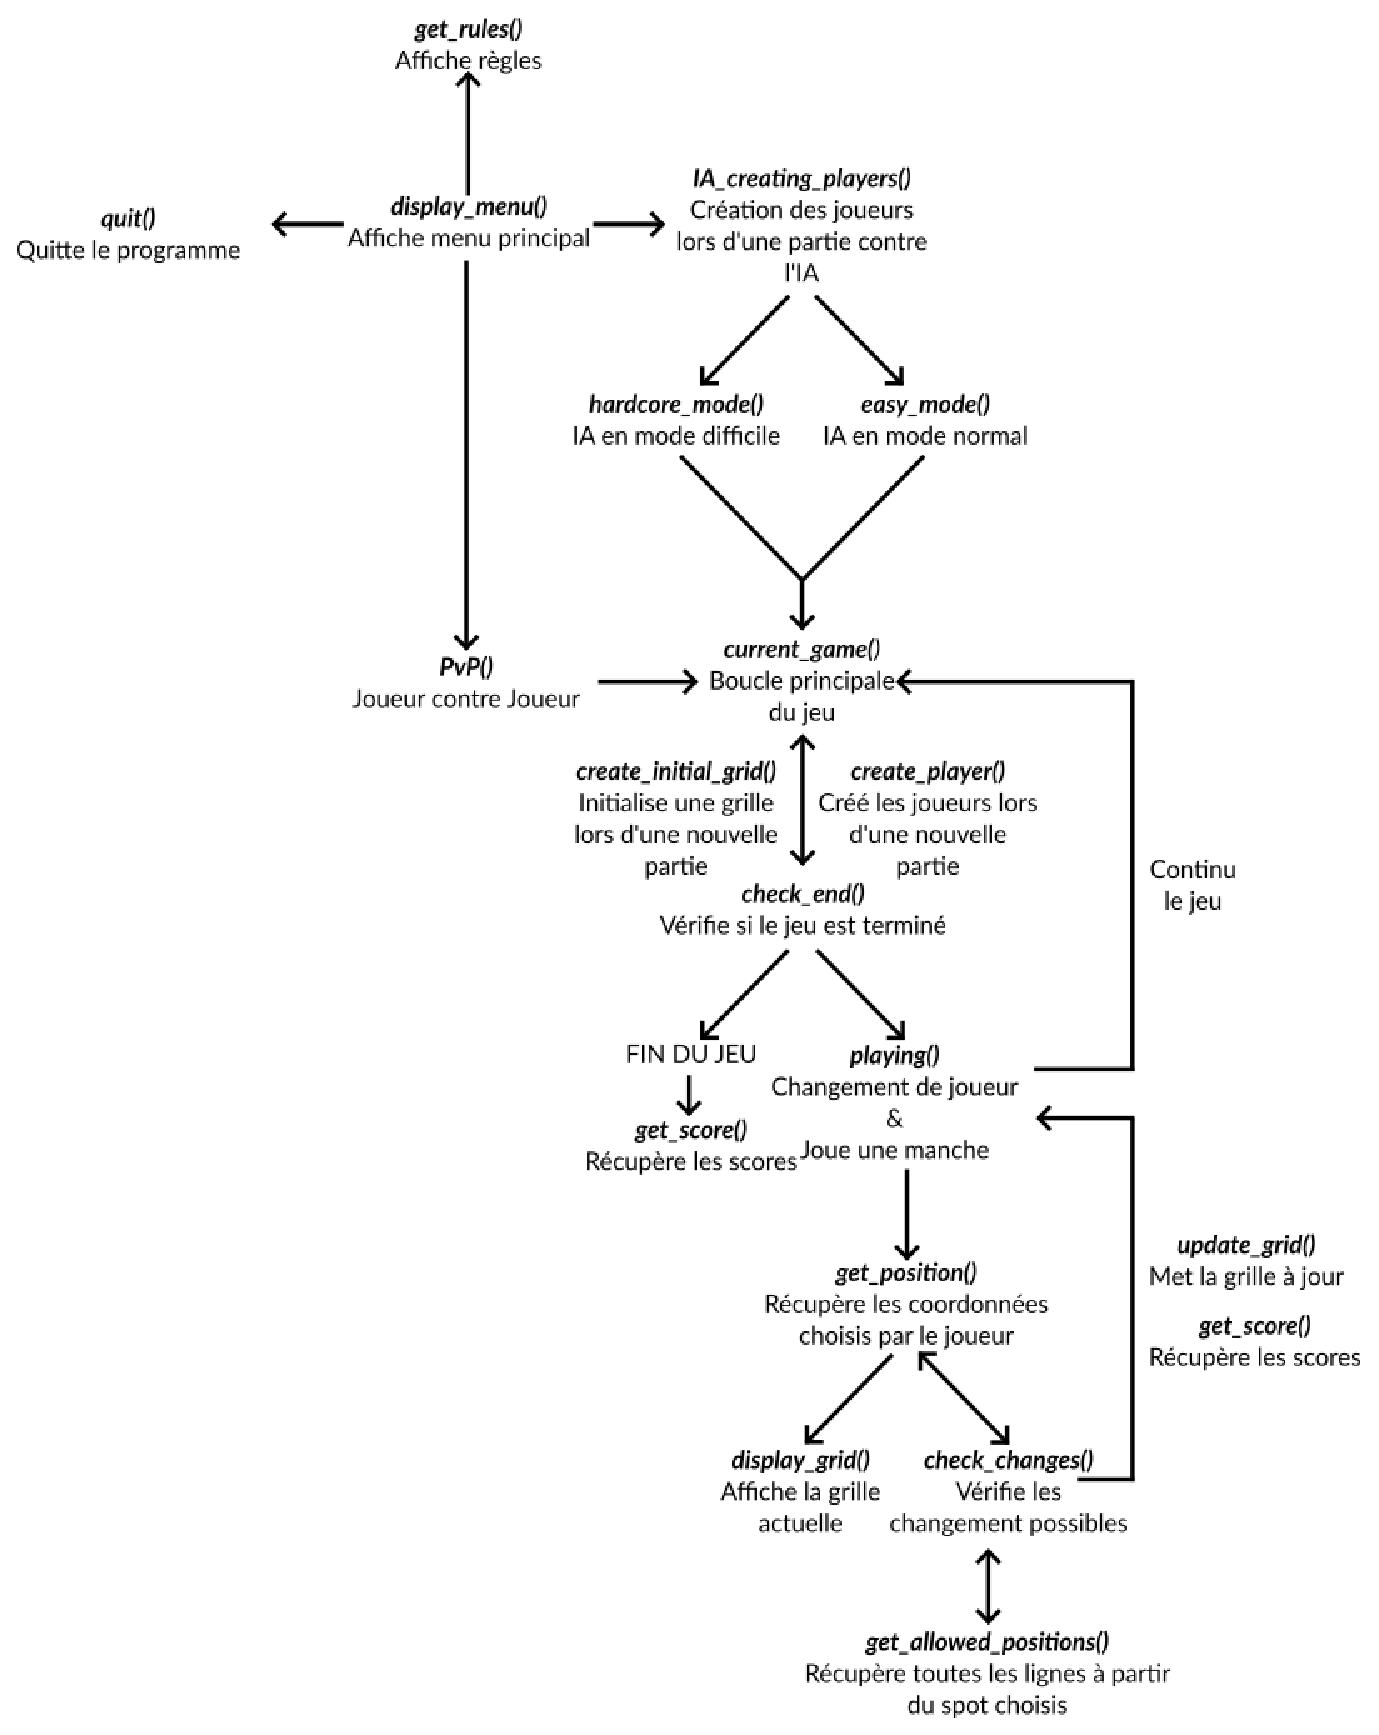
\includegraphics[scale=0.7]{flow.eps}

\end{document}